
\documentclass[11pt,a4paper]{article}
\usepackage[margin=1.7cm]{geometry}
\usepackage{amsmath,amssymb}
\usepackage{tikz}
\usepackage{xcolor}
\usepackage{parskip}
\usepackage[T1]{fontenc}
\usepackage[utf8]{inputenc}
\usepackage[dutch]{babel}
\usepackage{newtxtext,newtxmath}
\usetikzlibrary{arrows.meta,calc,positioning,decorations.pathmorphing}

\setlength{\parskip}{0.55em}
\setlength{\parindent}{0pt}

\newcommand{\uncertain}[1]{\textit{\textcolor{gray}{#1}}}

\title{Notebook 2012 --- Pagina's 48--50}
\author{}
\date{}

\begin{document}
\maketitle

\uncertain{Deze drie pagina's zijn visueel dicht en schetsmatig. De formules zijn zo letterlijk mogelijk overgenomen; bij moeilijk leesbare stukken is de meest waarschijnlijke lezing gekozen en expliciet als onzeker behandeld.}

\clearpage
\section*{Pagina 48}

\begin{minipage}[t]{0.48\textwidth}
\subsection*{Linkerhelft}
\textbf{Rotational Vortex}

\begin{center}
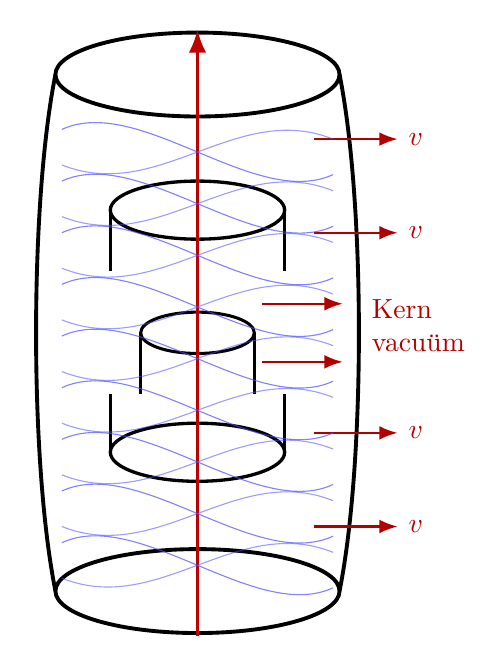
\begin{tikzpicture}[scale=0.82,>=Latex]
    % outer capsule
    \draw[black, line width=1.4pt] (0,4.0) ellipse (2.2 and 0.65);
    \draw[black, line width=1.4pt] (0,-4.0) ellipse (2.2 and 0.65);
    \draw[black, line width=1.4pt] (-2.2,4.0) .. controls (-2.6,2.0) and (-2.6,-2.0) .. (-2.2,-4.0);
    \draw[black, line width=1.4pt] (2.2,4.0) .. controls (2.6,2.0) and (2.6,-2.0) .. (2.2,-4.0);

    % inner disks / terraces
    \draw[black, line width=1.2pt] (0,1.9) ellipse (1.35 and 0.45);
    \draw[black, line width=1.2pt] (0,-1.85) ellipse (1.35 and 0.45);
    \draw[black, line width=1.1pt] (0,0.0) ellipse (0.88 and 0.32);
    \draw[black, line width=1.1pt] (-1.35,1.9) -- (-1.35,0.95);
    \draw[black, line width=1.1pt] (1.35,1.9) -- (1.35,0.95);
    \draw[black, line width=1.1pt] (-0.88,0.0) -- (-0.88,-0.95);
    \draw[black, line width=1.1pt] (0.88,0.0) -- (0.88,-0.95);
    \draw[black, line width=1.1pt] (-1.35,-1.85) -- (-1.35,-0.95);
    \draw[black, line width=1.1pt] (1.35,-1.85) -- (1.35,-0.95);

    % central flow
    \draw[red!75!black, very thick, ->] (0,-4.7) -- (0,4.7);
    % shell flows
    \foreach \y in {3.0,1.55,-1.55,-3.0}{
        \draw[red!70!black, thick, ->] (1.8,\y) -- (3.1,\y);
        \node[red!70!black, right] at (3.12,\y) {$v$};
    }
    \draw[red!70!black, thick, ->] (1.0,0.45) -- (2.25,0.45);
    \draw[red!70!black, thick, ->] (1.0,-0.45) -- (2.25,-0.45);

    % sketchy blue streamlines
    \foreach \yy in {-3.6,-2.8,...,3.6}{
      \draw[blue!70, opacity=0.7] (-2.1,\yy+0.35) .. controls (-0.9,\yy+0.9) and (0.9,\yy-0.9) .. (2.1,\yy-0.35);
      \draw[blue!70, opacity=0.55] (2.1,\yy+0.2) .. controls (0.6,\yy+0.8) and (-0.6,\yy-0.8) .. (-2.1,\yy-0.2);
    }

    \node[red!70!black, right, align=left] at (2.55,0.1) {Kern\\vacu\"um};
\end{tikzpicture}
\end{center}

\begin{align*}
v &= \frac{\Gamma}{2\pi R}
\\
R\,v &\approx \frac{\Gamma}{2\pi}
\end{align*}

Hoekmoment is constant.

\medskip
\uncertain{Onderste notitie: ``$v$ groeit niet recht evenredig met de radius''; in rood staat daaronder ``$v=\text{constant}$''.}
\end{minipage}
\hfill
\begin{minipage}[t]{0.48\textwidth}
\subsection*{Rechterhelft}
\textbf{Tijdruimte-buiging door een lading}

\begin{center}
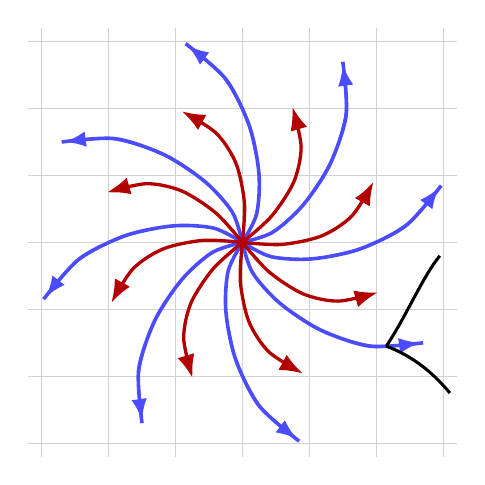
\begin{tikzpicture}[scale=0.85,>=Latex]
    % faint grid
    \foreach \x in {-3,-2,-1,0,1,2,3}{
        \draw[gray!35] (\x,-3.2) -- (\x,3.2);
    }
    \foreach \y in {-3,-2,-1,0,1,2,3}{
        \draw[gray!35] (-3.2,\y) -- (3.2,\y);
    }

    % blue spiral arms
    \foreach \a in {0,45,90,135,180,225,270,315}{
      \begin{scope}[rotate=\a]
        \draw[blue!70, line width=1.3pt]
          plot[smooth] coordinates {(0,0) (0.45,0.15) (0.9,0.55) (1.3,1.15) (1.55,1.9) (1.5,2.7)};
        \draw[blue!70, line width=1.0pt, ->]
          plot[smooth] coordinates {(1.05,0.75) (1.35,1.25) (1.55,1.95) (1.5,2.65)};
      \end{scope}
    }

    % red spiral arrows
    \foreach \a in {22,67,112,157,202,247,292,337}{
      \begin{scope}[rotate=\a]
        \draw[red!70!black, line width=1.2pt, ->]
          plot[smooth] coordinates {(0,0) (0.55,0.2) (1.05,0.55) (1.35,1.0) (1.45,1.6)};
      \end{scope}
    }

    % black bend
    \draw[black, line width=1.1pt] (2.15,-1.55) .. controls (2.45,-1.1) and (2.7,-0.5) .. (2.95,-0.2);
    \draw[black, line width=1.1pt] (2.15,-1.55) .. controls (2.55,-1.7) and (2.85,-1.95) .. (3.1,-2.25);
\end{tikzpicture}
\end{center}

\uncertain{Bovenaan staat waarschijnlijk: ``Ruimte buiging door een lading'' of ``Tijdruimte buiging door een lading''. De figuur toont een gedraaide spiraalvorm in een rooster.}
\end{minipage}

\clearpage
\section*{Pagina 49}

\begin{minipage}[t]{0.48\textwidth}
\subsection*{Linkerhelft}
\begin{align*}
f_e &= \frac{2 F_{\max} R_c C_e}{4\pi F_{\max} R_c^2}
\\
f_e &= \frac{C_e}{2\pi R_c}
\\
f_e &= \frac{8 \varepsilon_0 C_e F_{\max} R_c}{e^2}
\\
a_0 &= \frac{h}{2\pi m_e c \alpha}
\\
\alpha &= \frac{2 C_e}{c}
\\
a_0 &= \frac{h}{2\pi m_e c \left(\dfrac{2C_e}{c}\right)}
\\
a_0 &= \frac{h}{4\pi m_e C_e}
\\
h &= 4\pi m_e C_e a_0
\\
a_0 &= \frac{F_{\max} R_c^2}{m_e C_e^2}
\\
h &= 4\pi m_e C_e
     \left(\frac{F_{\max} R_c^2}{m_e C_e^2}\right)
\end{align*}

\[
h \approx \frac{4\pi F_{\max} R_c^2}{m_e\, c\, \alpha\, C_e}
\]
\uncertain{Onzekere lezing van de laatste, moeilijk leesbare regel.}

\uncertain{De laatste regel is lastig leesbaar en mogelijk een tussenvorm in de afleiding.}
\end{minipage}
\hfill
\begin{minipage}[t]{0.48\textwidth}
\subsection*{Rechterhelft}
\begin{align*}
a_0 &=
\left(\frac{4\pi F_{\max} R_c^2}{C_e}\right)
\left(\frac{1}{4\pi m_e C_e}\right)
\\[0.3em]
a_0 &=
\left(\frac{4\pi F_{\max} R_c^2}{C_e}\right)
\left(\frac{c^2}{8\pi F_{\max} C_e R_c}\right)
\\[0.3em]
h &\approx m_e c \lambda_e
\\
N_e &= \frac{2\pi c R_c}{C_e}
\\
m_e &= \frac{2 F_{\max} R_c}{c^2}
\\
N_e &= \frac{4\pi F_{\max} R_c^2}{C_e c m_e}
\end{align*}

{\color{green!50!black}
\begin{align*}
r^2 &\approx
\left(\frac{4\pi F_{\max} c^2}{C_e}\right)
\left(\frac{N}{8\pi^2 m_e f}\right)
\\
r^2 &= \frac{N h}{8\pi^2 m_e f}
\\
r^2 &\approx \frac{n^2 R_c}{4\pi C_e f}
\end{align*}
}

\medskip
\textbf{\color{red!70!black}Vortex Physics}

{\color{red!70!black}
\begin{align*}
\text{Vorticity:}\qquad
\frac{v}{R}\frac{dv}{dr} &= 2\vec{\omega}
\\
\text{\uncertain{[tweede grootheid]:}}\qquad
\frac{v}{R}\frac{dv}{dr} &\approx \alpha \vec{\omega}
\end{align*}
}

\uncertain{Rechts in rood staat een opmerking die waarschijnlijk ``velocity vast'' of ``$v/\gamma$'' aanduidt.}
\end{minipage}

\clearpage
\section*{Pagina 50}

\begin{minipage}[t]{0.48\textwidth}
\subsection*{Linkerhelft}
\begin{align*}
V_\theta(R,t)
&=
\frac{\Gamma}{2\pi R}
\left(
1-\exp\!\left(
-\frac{R^2}{R_c^2(t)}
\right)
\right)
\\[0.3em]
V_\theta
&=
\left(
1-e^{-R^2/(4\nu t)}
\right)
\frac{\Gamma}{2\pi R}
\end{align*}

Radius

Viscosity

\begin{align*}
R_c(t) &= \sqrt{4\nu t}
\end{align*}

\[
\Gamma = \text{circulaties binnen}
\]

\[
\text{Radial velocity}
\qquad \text{\uncertain{(schets van draaiende kring)}}
\]

\[
V_\theta(R)
=
V_{0\max}
\left(1+\frac{0.5}{\alpha}\right)
\frac{R_c}{r}
\left[1-\exp\!\left(-\alpha \frac{(\cdots)}{R}\right)\right]
\]
\uncertain{Deze regel is slechts gedeeltelijk leesbaar; de weergegeven vorm is de meest waarschijnlijke reconstructie.}

\[
\text{acceleratie} = -\omega^2 x
\]
\end{minipage}
\hfill
\begin{minipage}[t]{0.48\textwidth}
\subsection*{Rechterhelft}
\begin{center}
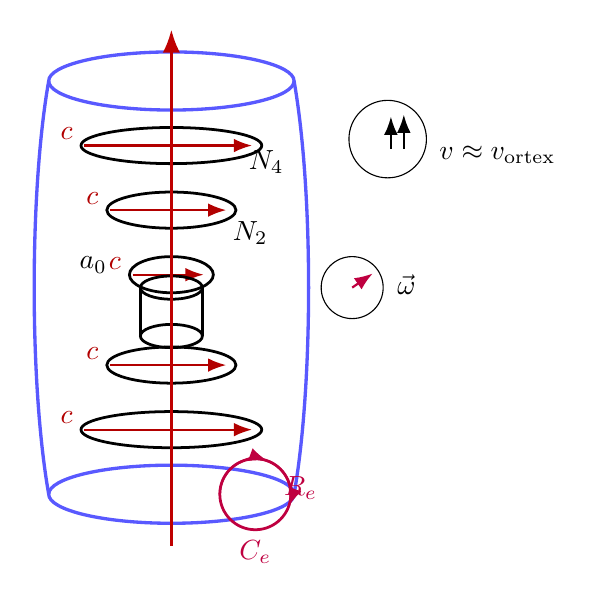
\begin{tikzpicture}[scale=0.82,>=Latex]
    % outer shell contour
    \draw[blue!65, line width=1.2pt] (0,3.2) ellipse (1.9 and 0.45);
    \draw[blue!65, line width=1.2pt] (0,-3.2) ellipse (1.9 and 0.45);
    \draw[blue!65, line width=1.2pt] (-1.9,3.2) .. controls (-2.2,1.5) and (-2.2,-1.5) .. (-1.9,-3.2);
    \draw[blue!65, line width=1.2pt] (1.9,3.2) .. controls (2.2,1.5) and (2.2,-1.5) .. (1.9,-3.2);

    % terraces
    \foreach \yy/\rad in {2.2/1.4,1.2/1.0,0.2/0.65,-1.2/1.0,-2.2/1.4}{
       \draw[black, line width=1.0pt] (0,\yy) ellipse ({\rad} and 0.28);
       \draw[red!70!black, thick, ->] ({-\rad+0.05},\yy) -- ({\rad-0.15},\yy);
       \node[red!70!black, left] at ({-\rad+0.02},{\yy+0.18}) {$c$};
    }

    % center core
    \draw[black, line width=1.0pt] (0,0) ellipse (0.48 and 0.18);
    \draw[black, line width=1.0pt] (-0.48,0) -- (-0.48,-0.75);
    \draw[black, line width=1.0pt] (0.48,0) -- (0.48,-0.75);
    \draw[black, line width=1.0pt] (0,-0.75) ellipse (0.48 and 0.18);
    \node[right] at (0.8,0.85) {$N_2$};
    \node[right] at (1.05,1.95) {$N_4$};
    \node[left] at (-0.85,0.35) {$a_0$};

    % vertical axis
    \draw[red!75!black, very thick, ->] (0,-4.0) -- (0,4.0);

    % small circles on right
    \begin{scope}[shift={(3.35,2.3)}]
        \draw[black] (0,0) circle (0.6);
        \draw[black, thick, ->] (0.05,-0.15) -- (0.05,0.35);
        \draw[black, thick, ->] (0.25,-0.15) -- (0.25,0.38);
        \node[right] at (0.65,-0.25) {$v \approx v_{\text{ortex}}$};
    \end{scope}
    \begin{scope}[shift={(2.8,0.0)}]
        \draw[black] (0,0) circle (0.48);
        \draw[purple, thick, ->] (0,0) -- (0.32,0.22);
        \node[right] at (0.55,0.05) {$\vec{\omega}$};
    \end{scope}
    \begin{scope}[shift={(1.3,-3.2)}]
        \draw[purple, line width=1.0pt] (0,0) circle (0.55);
        \draw[purple, thick, ->] (-0.55,0.0) arc[start angle=180,end angle=70,radius=0.55];
        \draw[purple, thick, ->] (0.0,0.55) arc[start angle=90,end angle=-20,radius=0.55];
        \node[purple] at (0,-0.9) {$C_e$};
        \node[purple] at (0.7,0.1) {$R_e$};
    \end{scope}
\end{tikzpicture}
\end{center}

{\color{purple}
\[
\text{vorticity} = 2\vec{\omega}
\qquad
\text{hoeksnelheid} = 2 C_e
\]
}

\uncertain{De rechterbladzijde toont een gestapelde vortexdoorsnede met labels $N_4$, $N_2$, $a_0$, meerdere snelheidsrichtingen $c$ en twee kleine rotatieschetsen.}
\end{minipage}

\end{document}
